\chapter{SPMonitor}

\todo{Add chapter introduction}

% This is the third result chapter which presents the first solution of the thesis. 
% The solution is integrated into the overall concept introduced in Chapter 4 and 
% it is technically based on the foundation described in Chapter 5.

% A thesis should provide at least two such solutions. 

\section{Analysis}
The components that will be chosen for SPMonitor must fulfill a few requirements.
These requirements are listed in Table \ref{tab:requirements}.
Firstly, the solution should be scaleable to an arbitrary amount of monitored instances, and different workload sizes.
Secondly, it should be possible to add new and different services in the future. This means that SPMonitor should be extensible.
Thirdly, the components license model must permit free commercial use.
Additionally, the components should be cloud agnostic, meaning that they are not bound to one vendor's specific cloud environment.
Similarly, the components should not depend upon specific choices for the other components, so that the whole system can be freely designed.

\begin{table}[h]
\begin{tabular}{l|l}
	& Requirement       			\\
\hline
R1 	& Scalability 					\\
R2 	& Extensibility       			\\
R3 	& License			  			\\
R4 	& Agnostic       				\\
\end{tabular}
\caption{Requirements for SPMonitor}
\label{tab:requirements}
\end{table}

\todo{Capabilities?}
\todo{Access Control/Roles/Security?}

\section{Design}

Note that the components are analyzed regarding their intended use.
The result is, that a component might be listed as not fulfilling a requirement even though it would be possible
to use the component in a way that fulfills the requirement. This is an important consideration for components
that are part of a complete monitoring stack that offers components for all three types of components.
Without this consideration, the fourth requirement would be violated.

\todo{Finish analysis of components}
% \begin{table}[]
% \begin{tabular}{l|c|c|c|c|l}
% Name 					& R1 & R2 & R3 & R4	& Note \\
% \hline
% Grafana 				& \cmark & \cmark & \cmark & \cmark & - \\
% Kibana 					& \cmark & \cmark & \cmark & \xmark & Part of the ElasticStack \\
% OpenSearch Dashboard 	& \cmark & \cmark & \cmark & \xmark & Part of the OpenSearch Project \\
% Apache SkyWalking 		& \cmark & \cmark & \cmark & \xmark & All-in-one solution 
% \end{tabular}
% \caption{Visualization Components}
% \label{tab:potential_visualization}
% \end{table}

% \begin{table}[]
% \begin{tabular}{l|c|c|c|c|l}
% Name 					& R1 & R2 & R3 & R4	& Note \\
% \hline
% Grafana Agent			& \cmark & \cmark & \cmark & \cmark & - \\
% Prometheus 				& \cmark & \cmark & \cmark & \cmark & - \\
% OpenSearch 				& \cmark & \cmark & \cmark & \cmark & - \\
% OpenTelemetry 			& \cmark & \cmark & \cmark & \cmark & - \\
% Apache SkyWalking 		& \cmark & \cmark & \cmark & \cmark & - 
% \end{tabular}
% \caption{Data Sources}
% \label{tab:potential_sources}
% \end{table}

% \begin{table}[]
% \begin{tabular}{l|c|c|c|c|l}
% Name 					& R1 & R2 & R3 & R4 & Note	\\
% \hline
% Prometheus 				& \cmark & \cmark & \cmark & \xmark & - \\
% ElasticSearch 			& \cmark & \cmark & \xmark & \xmark & - \\
% OpenSearch 				& \cmark & \cmark & \cmark & \xmark & - \\
% Apache SkyWalking 		& \cmark & \cmark & \cmark & \xmark & - 
% \end{tabular}
% \caption{Data Sinks}
% \label{tab:potential_sinks}
% \end{table}

The components that were chosen in the end, can be seen in Figure \ref{fig:sps_spmonitor}.
Grafana was chosen as the component for visualization together with Prometheus as the data source/sink.
The combination of Grafana with Prometheus is an industry-standard solution that offers a lot of flexibility
and functionality.
Because Prometheus only stores metrics in memory and does not provide long-term storage,
Grafana Mimir, with MinIO as a storage backend, was added to resolve this issue.
The Grafana Agent was added as an additional data source because it provides an easy method
of scraping performance metrics from Kubernetes Pods, which are then written to Prometheus for storage and analysis.

\begin{figure}
	\centering
	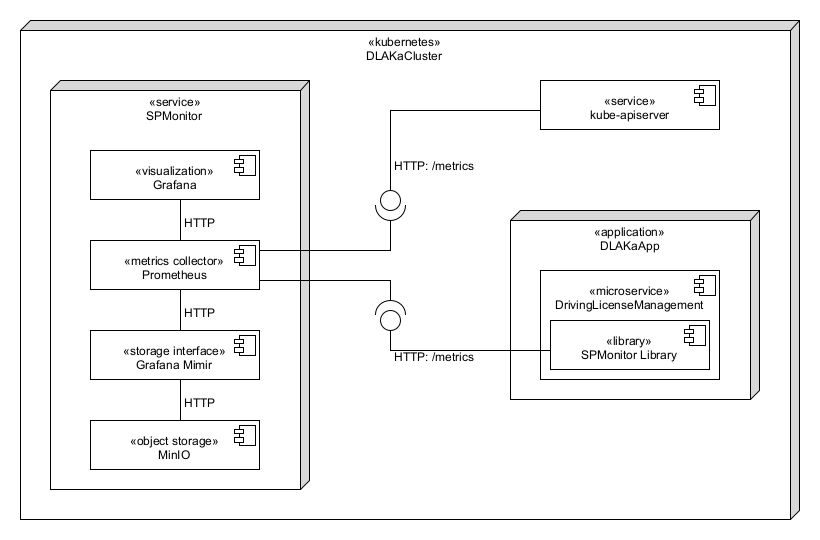
\includegraphics[width=\textwidth]{figures/sps_spmonitor.png}
	\caption{SystemPlusSoftware SPMonitor}
	\label{fig:sps_spmonitor}
\end{figure}

\section{Implementation}